\documentclass[11pt, a4paper, german]{article}

\usepackage{booktabs}
\usepackage{algorithmic}
\usepackage[titlenotnumbered, vlined, ruled]{algorithm2e}
\usepackage{amsfonts}
\usepackage{amsmath}
\usepackage{amssymb}
\usepackage{amsthm}
\usepackage{mathtools}

\usepackage{array}
\usepackage[ngerman]{babel}
\usepackage[utf8]{inputenc}
\usepackage{color}
\usepackage{enumerate}
\usepackage{graphicx}
\usepackage{hyperref}
\usepackage{latexsym}
\usepackage{pdflscape}
\usepackage{makecell}
\usepackage{makeidx}
\usepackage{multirow}
\usepackage{pdfpages}
\usepackage{tikz}
\usepackage{tkz-fct}
\usepackage{tkz-graph}
\usetikzlibrary{patterns}
\usepackage{upgreek}
\usepackage{standalone}
\usepackage{slantsc}
\usepackage{lmodern}
\usepackage[labelformat=empty, font={scriptsize}]{subcaption}
\usepackage[labelformat=empty, font={scriptsize}]{caption}
\usepackage{pgfplots}
\usepackage{pgfplotstable}
\usepackage{circuitikz}
\usepackage{changepage}

\usetikzlibrary{shapes}
\usetikzlibrary{matrix, arrows,fit,shapes.gates.logic.US,shapes.gates.logic.IEC,calc,backgrounds,decorations.pathmorphing}




\DeclarePairedDelimiter\abs{\lvert}{\rvert}
\makeatletter
\let\oldabs\abs
\def\abs{\@ifstar{\oldabs}{\oldabs*}}
%
\let\oldnorm\norm
\def\norm{\@ifstar{\oldnorm}{\oldnorm*}}
\makeatother

\newcommand{\area}{\text{area}}
\newcommand{\uniquecone}{\text{unique\_cone}}
\newcommand{\uniquearea}{\text{unique\_area}}

\pgfplotsset{compat=1.8}

%
% Colors
%
\definecolor{darkblue}{RGB}{10, 0, 128}
\definecolor{grey}{RGB}{128, 128, 128}
\definecolor{darkred}{RGB}{180, 0, 0}
\definecolor{darkgreen}{RGB}{0, 100, 0}
\definecolor{lightgrey}{RGB}{210,210,210}
\newcommand{\RED}[1]{\textcolor{darkred}{#1}}
\newcommand{\BLUE}[1]{\textcolor{darkblue}{#1}}
\newcommand{\GREEN}[1]{\textcolor{darkgreen}{#1}}
\renewcommand{\emph}[1]{{\BLUE{#1}}}

\definecolor{darkRed}{rgb}{0.6,0,0}
\definecolor{lightRed}{rgb}{1,0.75,0.75}
\definecolor{darkGreen}{rgb}{0,0.5,0}
\definecolor{PineGreen}{rgb}{0.01,0.5,0.45}
\definecolor{darkBlue}{rgb}{0, 0, 0.75}
\definecolor{CornflowerBlue}{rgb}{0.15,0,0.7}
\definecolor{lightBlue}{rgb}{0.75,0.75,1}
\definecolor{grey}{rgb}{0.5,0.5,0.5}
\definecolor{black}{rgb}{0,0,0}
\definecolor{red}{rgb}{1,0,0}
\definecolor{green}{rgb}{0, 0.8, 0.3}
\definecolor{blue}{RGB}{10, 0, 128}
\definecolor{yellow}{rgb}{1,1,0}
\definecolor{orange}{rgb}{1,0.6,0}
\definecolor{cyan}{rgb}{0,0.7,1}
\definecolor{purple}{rgb}{0.5,0,0.8}

\newcommand\mycommfont[1]{\footnotesize\ttfamily\textcolor{darkGreen}{#1}}{}{}
\SetCommentSty{mycommfont}
\SetArgSty{textup}
\renewcommand\thempfootnote{\arabic{mpfootnote}}
\renewcommand{\thealgocf}{}

% \SetKwComment{Comment}{}{}

%
% Shorthands
%
\newcommand{\BL}{\textsc{BonnLogic}}
\newcommand{\Restr}{\textsc{And-Or}-Path Restructuring}
\newcommand{\AOP}{\textsc{And-Or}-Path}
\newcommand{\aop}{\textsc{And-Or}-path}

% \pgfpagesuselayout{resize to}[a4paper,landscape,border shrink=5mm]

% CONFIGURE PACKAGES

% NEW COMMANDS

\newcommand{\bl}[1]{\index{BonnLogic@\textsc{BonnLogic}!#1}}

\newcommand{\brent}[1]{\index{Brents adder@Brent's adder!#1}}

\newcommand{\ceil}[1]{\left\lceil #1 \right\rceil}

\newcommand{\delay}{\mathrm{delay}}

\newcommand{\depth}{\mathrm{depth}}

\newcommand{\floor}[1]{\left\lfloor #1 \right\rfloor}

\newcommand{\ld}{\log_{2}}

\newcommand{\loq}{\log_{\phi}}

\newcommand{\mini}[4]{\begin{minipage}{#1\linewidth}#3\end{minipage}\hfill\begin{minipage}{#2\linewidth}#4\end{minipage}}

\newcommand{\minialt}[4]{\centering{\begin{minipage}{#1\linewidth}#3\end{minipage}\begin{minipage}{#2\linewidth}#4\end{minipage}}}

\newcommand{\myindex}[1]{\emph{#1}\index{#1}}

\newcommand{\npfx}[1]{\index{non-prefix adders!#1}}

\newcommand{\OPT}{\mathrm{OPT}}

\newcommand{\pfx}[1]{\index{parallel prefix graph!#1}}

\newcommand{\size}{\mathrm{size}}

\newcommand{\sset}[1]{\left\{#1\right\}}

\newcommand{\todo}[1]{
  %\textcolor{red}{(TODO: \emph{#1})}
}

\newcommand{\vare}{\varepsilon}


% IMAGES

\newcommand{\tikzs}[2]{
  \centering
  \includegraphics[width=#1\linewidth]{images/#2.pdf} %fast
  %\ttikz{#2.tex}{#1} %slow
}
\newcommand{\tikzc}[3]{
  \centering{
    \includegraphics[width=#2\linewidth]{images/#3.pdf}
    \caption{#1}
    \label{fig:#3}%
  }
}
\newcommand{\tikzcc}[3]{
  \centering{
    \resizebox{#2\linewidth}{!}{
      \begin{tikzpicture}
        \input{images/#3}
      \end{tikzpicture}
    }
    \caption{#1}
    \label{fig:#3}%
  }
}
\newcommand{\ntikz}[1]{
  \begin{tikzpicture}
    \input{images/#1}
  \end{tikzpicture}
}
\newcommand{\ttikz}[2]{
  \centering{
    \resizebox{#2\linewidth}{!}{
      \begin{tikzpicture}
        \input{images/#1}
      \end{tikzpicture}
    }
  }
}
\newcommand{\ttikzfig}[3]{
  \begin{figure}[hbt]
    \centering{
      \resizebox{#2\linewidth}{!}{%
        \begin{tikzpicture}
          \input{images/#3}
        \end{tikzpicture}%
      }%
    }%
    \caption{#1}
  \end{figure}
}
\newcommand{\tikzfigs}[3]{
  \begin{figure}[hbt]%
    \centering{%
      \includegraphics[width=#2\linewidth]{images/#3.pdf}
      \caption{#1}%
      \label{fig:#3}%
    }%
  \end{figure}%
}
\newcommand{\tikzfigsc}[3]{
  \begin{figure}[hbt]%
    \centering{%
      \resizebox{#2\linewidth}{!}{%
        \begin{tikzpicture}
          \input{images/#3}
        \end{tikzpicture}%
      }%
      \caption{#1}%
      \label{fig:#3}%
    }%
  \end{figure}%
}
\newcommand{\tikzfig}[2]{
  \tikzfigs{#1}{1}{#2}
}


\usepackage{standalone}
\usepackage{slantsc}
\usepackage{lmodern}
%\newcounter{algorithm}
%\newtheorem{algorithm}[algorithm]{Algorithm}

\theoremstyle{plain}
\newtheorem{theorem}{Theorem}[section]
\newtheorem{cor}[theorem]{Corollary}
\newtheorem{lemma}[theorem]{Lemma}
\newtheorem{conj}[theorem]{Conjecture}
\theoremstyle{definition}
\newtheorem{definition}[theorem]{Definition}
\theoremstyle{remark}


\usepackage{caption}
\usepackage{subcaption}
\clubpenalty = 10000
\widowpenalty = 10000 
\displaywidowpenalty = 10000
\usepackage{Titelseite}
\usepackage{bbold}
\usepackage{graphicx}
\newcommand{\TM}{TechnologyMapping }

%Namen des Verfassers der Arbeit
\author{Alexander Zorn}
%Geburtsdatum des Verfassers
\geburtsdatum{26. Mai 1996}
%Gebortsort des Verfassers
\geburtsort{Bonn}
%Datum der Abgabe der Arbeit
\date{\today}

%Name des Betreuers
% z.B.: Prof. Dr. Peter Koepke
\betreuer{Betreuer: Prof. Dr. Stephan Held}
%Name des Instituts an dem der Betreuer der Arbeit tätig ist.
\zweitgutachter{Zweitgutachter: YYYY YYYY}
%z.B.: Mathematisches Institut
\institut{Forschungsinstitut f\"ur Diskrete Mathematik}
%Titel der Bachelorarbeit
\title{Heuristiken f\"ur das TechnologyMapping}
%Do not change!
\ausarbeitungstyp{Bachelorarbeit Mathematik}



\begin{document}

\maketitle

\tableofcontents
\newpage 
\section{Einleitung}

Der zunehmende Gebrauch elektronischer Geräte verlangt nach immer leistungsfähigeren Computerchips. Ein solcher wenige Quadratzentimeter große Chip beherbergt bis zu mehreren Milliarden Transistoren, welche, durch Drähte verbunden, gemeinsam eine Logische Funktion errechnen. Das Chipdesign beschreibt die Aufgabe aus einer gegeben Logischen Funktion einen herstellbaren Chip zu entwerfen, welcher diese Funktion realisiert. \\ 
\begin{wrapfigure}{r}{6cm}
	\scalebox{1}[-1]{
		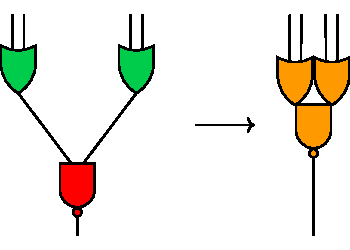
\includegraphics[]{pictures/compiled/einfBsp}
	}
		\caption{Zwei Realisierungen der Logischen Funktion $\neg((w\lor x) \land (y \lor z))$}
\end{wrapfigure}
Mithilfe von, aus wenigen Transistoren konstruierten, Bauteilen (genannt Gates, z.B.: AND, OR, INV, OAI) lässt sich eine Logische Funktion nachbilden. Abbildung 1 (links) zeigt dies an einem kleinen Beispiel.  Die Realisierung einer solchen Funktion ist jedoch nicht eindeutig, wie die in Abbildung 1 (links und rechts) gezeigte Nachbildung, beweist. \\
Die Größe der Menge aller möglicher Baupläne (später Circuit) für eine Logische Funktion hängt maßgeblich von der Anzahl der zur Verfügung stehenden Bauteile, sowie von dem Aufbau der Funktion, ab.
Es stellt sich heraus, dass im Allgemeinen eine Vielzahl möglicher Realisierungen einer Logischen Funktion existieren. Jedes Bauteil besitzt physikalische Eigenschaften an Größe, Geschwindigkeit (Delay) etc.. Somit besitzt auch jede Realisation solche Eigenschaften. \\
Ziel des \TM ist es für eine Logische Funktion eine Realisierung zu finden, welche eine Kostenfunktion (bestehend aus den physikalischen Eigenschaften) optimiert. Die Wahl der Implementierung hat direkte Auswirkungen auf die  Schnelligkeit, Größe und den Stromverbrauch des fertigen Chips. Hierbei geht das \TM von einer bereits realisierten Logischen Funktion aus und baut diese um zu einer möglichst kostengünstigen Alternative um. \\
Der optimale mögliche Umbau lässt sich bei kleinen oder eingeschränkten gegebenen Bauplänen noch in akzeptabler Zeit finden. Die Lösung dieses Problem für allgemeine Baupläne und Kostenfunktionen ist jedoch ein NP vollständiges Problem. Aus diesem Grund entwickelt die folgende Arbeit eine Heuristik, welche für sehr (mehrere 10.000 Bauteile) große Baupläne in akzeptabler Zeit einen möglichst kostengünstigen Umbau ermöglicht.
\newpage

\section{Terminologie \& grundlegender Algorithmus}
\subsection{grundlegende Definitionen}
Es folgen ein paar grundlegende Definitionen zur Beschreibung des Problems.

\begin{definition}{Boolesche Variable und Funktion: } \\
Eine boolesche Variable ist eine Variable mit Werten in $ \{ 0 , 1 \} $.
Sei $ n, m \in \mathbb{N}$. Eine boolesche Funktion ist eine Funktion $ f : \{ 0 , 1 \}^n \rightarrow \{ 0 , 1 \}^m $ mit n inputs und m outputs. 
\end{definition}

\begin{definition}{Gate und Library:}\\
Ein Gate $g$ mit Eingangsgrad $ n \in \mathbb{N}$ ist ein Tripel $(f_g, d_g, area_g)$. Hierbei sind $d_g, area_g \in \mathbb{R}_{\geq 0}$. Des Weiteren gilt $f_g$ ist eine boolesche Funktion mit $ f_g : \{0,1\}^n \rightarrow \{0, 1\} $. \\
Eine Library L ist eine Menge von Gates und sei \\ 
$fanin_{max} := max\{ arity(g) | g \in L \}$.
\end{definition}
\begin{figure}[h]
\begin{center}
 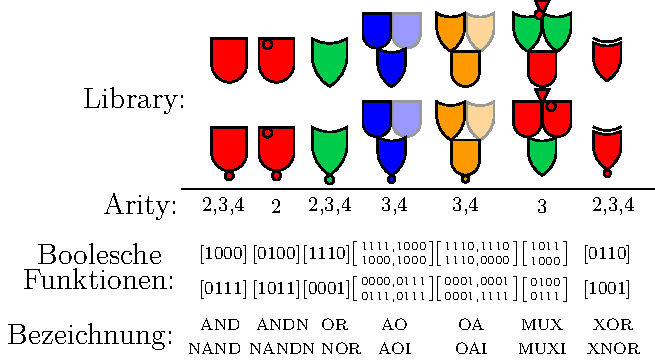
\includegraphics[height = 80pt]{./pictures/compiled/new_library.pdf}
 \caption{Beispiel einer Library}
 \label{fig:bsplib}
\end{center}
\end{figure}
$area_g$ gibt die Größe des physikalischen Bauteils an und $d_g$ beschreibt die Zeit die ein Signal braucht um von den inputs des Gates zu seinem Output zu gelangen. Dieser Wert lässt sich noch weiter differenzieren indem man $d_g \in \mathbb{R}^n$ wählt und somit Zeiten für jeden der Inputs angeben werden kann.\\

\begin{definition}{Circuit:}\\
Ein Circuit ist ein gerichteter kreisfeier Graph (directed acyclic graph DAG) mit folgenden Eigenschaften. Jeder Knoten gehört zu einer der aufgelisteten Kategorien: 
\begin{itemize}
\item{\bf Input} Knoten mit Eingangsgrad Null.
\item{\bf Gates} mit mindestens einer eingehenden Kante und ausgehenden Kante. Diese korrespondieren zu der Definition oben mit dem Zusatz dass an jedem der Inputs optional ein Inverter liegen kann.
\item{\bf Outputs} mit genau einer eingehenden Kante und keiner ausgehenden.
\end{itemize}
Ein Gate mit mehr als einer ausgehenden Kante wird auch Highfanoutgate genannt.\\
Ein Circuit realisiert durch Verschachtelung der booleschen Funktionen seiner Gates ebenfalls eine boolesche Funktion. \\
Zwei Circuits heißen äquivalent, wenn sie die gleiche boolesche Funktion realisieren.
\end{definition}

In einem Circuit lassen sich Teilgraphen durch ein Gate der Library austauschen. Voraussetzung für einen solchen Tausch ist, dass der veränderte Circuit äquivalent zu dem originalen ist. Dies sicher die folgenden Definitionen. 

\begin{definition}{Match und Kandidat:}\\
Sei g ein Gate in einem Circuit $C$. Ein (invertiertes) Match m ist ein Tupel $(p_m, I_m, f_m, inv_m)$ welches folgendes enthält:
\begin{itemize}
\item Ein Gate p der Library
\item Eine Menge X von Knoten aus der Circuit und eine Bijektion $ f: X \rightarrow inputs(p)$
\item Ein Funktion $ inv : inputs(p) \rightarrow \{not\_inv , inv \}$
\end{itemize}
So dass der Circuit $C'$, welcher durch den Austausch des Sub-Circuits von X bis g durch das Match (mit den durch inv definierten Invertern an den Inputs) entsteht, äquivalent zu C ist.
Ein invertiertes Match auf g ist ein Match auf g mit einem Inverter an jedem seiner Outputs.\\
Ein (invertierter) Kandidat auf g besteht aus einem (invertierten) Match auf g und einem Kandidaten für jeden Input Knoten von g (welcher kein Input von C ist).
\end{definition}

\begin{definition}{Circuit-Kandidat:}
Sei C ein Circuit mit Outputknoten Menge O. Eine Circuit-Kandidat K von C ist eine Menge von Kandidaten, sodass $\forall o \in O \, \exists!  h  \in K : h$ ist Kandidat von $ o$ und an jedem Knoten von C an dem sich mehrere Kandidaten überschneiden ist dasselbe Match gewählt.
\end{definition}
Folgendes Beispiel visualisiert die vorherigen Definitionen.\\
BILD EINSETZEN

Ein Circuit-Kandidat C ist eine Möglichkeit den Circuit physikalisch zu realisieren. Wie bereits in der Einleitung bemerkt gilt es nun den besten Kandidaten auf C auszuwählen. Dafür ist ein Maß für Implementierungen von Circuits notwendig. Es folgen zwei geläufige Beispiele. In der Praxis (und im späteren Verlauf dieser Arbeit) wird in der Regel eine convex-Kombination aus beiden verwendet.

\begin{definition}{Area und Delay eines Kandidaten:}\\
Sei C ein Circuit und K ein Circuit-Kandidat auf C. Dann gilt: \\
\begin{itemize}
\item $area(K) = \sum_{g \in gates(C)} (a_g + \sum_{i \in inputs(g)} \mathbb{1}_{\{inv_g(i)==inv\}} area_{inv})$ \\
wobei $area_{inv}$ die Größe eines Inverters ist.
\item $AT(K) = $\\$  \max\limits_{k \in can(K)} \{\max\limits_{i \in inputs(k)} \{   d_{gate(k)} + \mathbb{1}_{\{inv_g(i)==inv\}} d_{i} + AT(inp\_can(k,i)) + d_{w(k,i)} \} \}$ 
\end{itemize}
Wobei $can(K)$ die Menge der Kandidaten von $K$ sind und $inputs(k)$ sind die Inputknoten des Outputknoten des Kandidaten k. Des Weiteren ist $d_i$ das Delay eines Inverters und $d_{w(k,i)} $ das Delay der Kante zwischen den Knoten $k$ und $i$. $inp\_can(k,i)$ gibt den Kandidaten des $i$'ten Inputs von k zurück. 

\end{definition}

Das Delay (AT) gibt an wann das letzte Signal aus einem der Outputs des Circuit kommt.

\subsection{Kern Algorithmus}

Es folgt ein grundlegender Algorithmus, welcher auf eingeschränkten Circuits arbeitet, jedoch im weiteren Verlauf dieser Arbeit zu einer Heuristik für allgemeine sehr große Circuits erweitert wird.

\begin{problem}[framed]{(einfaches) Technology Mapping}
  Instanz:  & Circuit $C$ ohne Highfanoutknoten (Knoten mit nur einer ausgehenden Kante), mit eindeutigem Output $o$, Library $L$ mit beschr\"anktem $fanin_{max}$\\
  Aufgabe: &  Finde einen Kandidaten $K$ auf $o$, welcher die Arrivaltime/Area minimiert.
\end{problem}

\begin{algorithm}[H]
 \LinesNumbered
 \DontPrintSemicolon
 \caption{(einfaches) Technology Mapping}
 \SetKwInOut{Task}{Task}
 \KwIn{Circuit $C$ kreisfrei mit finalem Output $o$, Library $L$}

 bester\_kandidat[] $\gets \emptyset$\;
 bester\_inv\_kandidat[]$ \gets \emptyset$\;
 \ForEach{Knoten $v \in V(G)$ in topologischer Reihenfolge}
 {
   berechne alle (invertierten) Matches auf $v$\;
   \ForEach{ Match $m$ auf $v$ }
   {
      Berechne besten Kandidaten mit $m$ auf $v$\;
      Update best\_(inv)\_kandidaten\;
   }
 }
 Implementiere $C$ entsprechend bester\_kandidat[$o$]\;
\end{algorithm}\ \\

Dieser geht in topologischer Reihenfolge durch die Knoten v des Graphen und berechnet alle Matche auf v. Diese Matche werden dann zu einem Kandidaten ergänzt. Dieser Schritt (6) lässt sich sehr schnell implementieren, da für jedes Match m die besten Kandidaten der Inputs von m bereits bekannt sind.\\
 Ohne Highfanout-Knoten überschneiden sich diese nicht, und der beste Kandidat (inklusive der invertierten Verisonen) für jedes Match ist schnell gefunden. Von diesen wird der beste (in Bezug auf Area oder Arrivaltime) in Schritt 7 zu zur Liste der besten Kandidaten hinzugefügt.\\
 
\begin{cor}{Das (einfache) \TM besitzt \\ $\mathcal{O}(  |V(C)||L| fanin_{max})$-Laufzeit}\\
 	  Schritt 1 und 2 besitzen Laufzeit $\mathcal{O}(1)$. Schritt 4 lässt sich in \textcolor{red}{ wielange braucht es ein zu checken ob ein gate der Library ein Match eines Knoten sein kann ? ? plus Begründung! Laufzeit anpassen}. Schritt 6 ist wie bereits erwähnt schnell implementierbar, da für jeden der max $fanin_{max}$ Inputs der beste Kandidat verlinkt werden muss. Die Invertierten Matche werden nur gebarucht wenn der Input invertiert war. Somit braucht $\mathcal{O}(fanin_{max})$. Schritt 3 und 5 sind zwei verschachtelten Schleifen mit  $|V(C)|$ und max $|L|$ Durchläufen. \\
Daraus folgt eine Laufzeit von $\mathcal{O}(  |V(C)||L| fanin_{max})$. \hfill $\Box$
\end{cor}


\newpage
\section{Allgemeiner Algorithmus und Heuristik}
\subsection{Tradeoffprobleme}
Der oben vorgestellte Algorithmus ist in der Lage den bestmöglichen Umbau eines eingeschränkten Circuits zu bezüglich Area oder Delay zu errechnen. \\
Es existiert  ein Tradeoff zwischen beiden Area und Delay. Dies hat zur Folge, dass ein möglichst kleiner Circuit im Allgemeinen sehr langsam ist und man bei einer sehr schnellen Lösung mit einem großen Platzverbrauch rechnen muss. In der Anwendung des \TM ist jedoch weder ein sehr langsamer noch ein besonders grosser Circuit akzeptabel. Daraus folgt die Nachfrage nach einem Algorithmus, welcher in der Lage ist bezüglich einer Konvexkombination oder einer Schranke zu optimieren. Daraus ergeben sich die beiden folgenden Optimierungs-Probleme: \\
\textcolor{red}{Hier beide Probleme einfügen}\\


Diese \textcolor{red}{diese Probleme sind äquvalent Beweis? oder verweis aus quelle}
\textcolor{red}{erwähnen dass da die äquivalent sind von nun an nur noch die Konvexkombination verwendet wird}

Dadurch ergibt sich folgende Problemstellung für den Algorithmus: An jedem Knoten v lässt sich jetzt nicht mehr nur der Kandidat speichern, welche die Kostenfunktion an v optimiert. Angenommen v liegt in einem sehr Delay kritischen Gebiet des Graphen, dann kann es sehr gut sein dass es für einen Nachfolger von v sehr günstig ist v vollständig auf Delay hin zu optimieren und seine Kosten zu verbessern, was jedoch nicht möglich ist wenn der einzige an v gespeicherte Kandidat dieser ist der die Kosten ( Konvexkombination) an optimiert. \textcolor{red}{diesen satz verbessern!}\\
Die Kosten eines Kandidaten k sind somit nicht $\lambda AT(k) +(1-\lambda )area(k)$,  sondern das Tupel $(AT(k), area(k))$.
Es gibt jedoch eine Klasse von Kandidaten, welche nicht gespeichert muss. Dazu folgende Definition\\

\begin{definition}{(dominierte Kandidaten)}\\
	Seien $k_1, k_2$ Kandidaten desselben Knotens. Dann wird $k_1$ von $k_2$ dominiert, wenn gilt:\\
	$AT(k_1) < AT(k_2) und area(k_1) \leq area(k_2)$\\
	$	AT(k_1) \leq AT(k_2) und area(k_1) < area(k_2)$\\	
\end{definition}

Eine optimale Lösung des \TM verwendet offenbar (\textcolor{red}{in einem Korollar beweisen ?}) nur nicht-dominierte Kandidaten, woraus folgt, dass nur diese während der Ausführung des Algorithmus gespeichert werden müssen.\\
Die Menge der noch bleibenden Kandidaten lassen sich in sogenannten Tradeoff-Kurven speichern (siehe Abbildung ?? \textcolor{red}{Abbildung hinzufügen.. kann ich Lucas verwenden ?}). Welche jeden Kandidaten zweidimensional anhand seiner Kosten erfasst.


\textcolor{red}{Next things todo: Algorithmus erweitern und dann auf die Filterung mit Buckets eingehen inclusive der funktionierenden epsilon betrachtung -> ohne beweis mit erklärung\\ 
angenommen ich lasse den algo hier weg und mache highfanout sowie RAts vorher vorher und dann am ende des Kapitel kommt der zusammenfassende Algorithmus und daraus dann mit buckets filterung erklärung etc die heuristik???}


\subsection{Highfanoutknoten}
Der oben beschriebene Kern Algorithmus arbeitet nur auf Circuits, in denen keine Highfanoutknoten existieren. Diese Eigenschaft kommt auf einem realen Chip jedoch sehr häufig vor(\textcolor{red}{prozent Zahl herausfinden und einsetzen (verlinkung auf Analysen und Test Kapitel)}). Es ist möglich einen Circuit, in kleinere Subcircuits zu unterteilen, welche solche HIghfanoutknoten nicht besitzen. Die Subcircuits werden daraufhin einzeln mit dem Algorithmus (sehr schnell) optimiert und daraufhin zu einem C äquvalenten Circuit C' zusammengesetzt. Diese Vorgehensweise findet sich ausführlich in \textcolor{red}{Hier das eine Paper suchen plus einfügen} wieder. Die folgende Abbildung verbildlicht diesen Ansatz einer Heuristik. \textcolor{red}{Bild erstellen, welches sich an dem des Papers orientiert}. Der Anteil an Highfanoutknoten ist auf den mir vorliegenden Chips so groß, dass eine vielzahl sehr kleiner Subcircuits mit einer somit sehr kleinen Anzahl an Kandidaten, woraus folgt, dass die Möglichkeiten des \TM sehr eingeschränkt werden. Aus diesem Grund werde ich auf diese Art der   Heuristik nicht mehr eingehen. \textcolor{red}{kann man das so schreiben ?}\\

\textcolor{red}{Klonen erwähnen? (aktuell wird sie nicht erwähnt}\\
Das Kern-Problem der Highfanoutknoten ist, dass bei der Konstruktion des äquvalenten Circuits die Kandidaten aller Nachfolger eines Highfanoutknoten v an v übereinstimmen müssen. Daraus folgt, das bei der Wahl eines Kandidaten für einen Knoten w die Wahl der Kandidaten der Input-Kandidaten von w nicht unabhängig von einander sein muss. \\
Zur Lösung des Problems helfen die folgenden Definitionen:\\

\begin{definition}{cone}\\
	Sei C ein Circuit und v ein Knoten von C. Dann sei die cone von v: 
	\[ cone(v) := C[V \cup \{ v \}], V = \{ w \in V(C) : \exists \text{ w-v-Weg in }  C \} \] 
\end{definition}
\textcolor{red}{Bild ? }

\begin{definition}
	Sei C ein Circuit und  $v \in V(C)$. Dann wird die durch $cone(v)$ berechnete Funktion. Die 			{\bf bis v berechnete Funktion} genannt.
\end{definition}

\textcolor{red}{einheitlich mit Absätzen in definitionen mach es einfach wie lukas !}

\begin{definition}{offene Knoten}\\
	Sei $C$ ein Circuit und $v,w \in V(C)$. Dann heißt $w$ offener Knoten von $v$, wenn folgendes gilt: 
	\[ w \in cone(v)\backslash \{ v \} \text{ und } | \delta ^{+}(w)| \geq 2 \text{ und } \exists o \in V(C) \backslash cone(v) : \exists \text{ w-o-Weg in } C \] 	
\end{definition}
Mit anderen Worten ist die Menge der Offenen Knoten eines Circuit Knoten v, die Menge aller Highfanoutknoten w, von welchen aus man sowohl v als auch einen Knoten außerhalb der Cone von v erreichen kann. Von dieser Menge ist v selber ausgenommen. Dies sind gerade die Highfanout-Knoten, welche durch die Kandidaten eines Knoten außerhalb von $cone(v)$ verändert werden können. Alle Kandidaten von  Knoten mit Ausgangsgrad 1 und dieser Eigenschaft, sind durch den Nachfolger-Kandidaten (welcher auch zu einem offene Knoten gehören muss), bereits eindeutig definiert. \textcolor{red}{Formulierung?} \\

\begin{definition}{Klasse eines Kandidaten}\\
	Sei $k$ ein Kandidat auf einem Knoten $v$ und $O$ die Menge der offenen Knoten von $v$. Die Klasse $class(k)$ ist eine Abbildung, welche jedem Element $w \in O$ den durch $k$ festgelegten Kandidaten auf $w$ zuordnet.\\
\end{definition}
Nach der einführenden Erläuterung lassen sich zwei Kandidaten $k_1,k_2$ eines Knoten $v$ mit $class(k_1) \neq class(k_2)$ nicht miteinander vergleichen. Dies gilt auch für den Fall, wenn $k_2$ von  $k_1$ dominiert wird, denn es ist möglich, dass dies zwar an der Stelle $v$ gilt, jedoch nicht an allen offenen Knoten von $v$. Daraus folgt würde man $k_2$ löschen, so löscht man evtl den besten Kandidaten des Outputs von C. \\
Um somit mit Highfanoutknoten arbeiten zu können, werden für jeden Knoten $v$ und jede Klasse von $v$ ,in dem exakten Algorithmus, alle nicht dominierten Kandidaten gespeichert. Daraufhin wird ist der noch verbleibende beste Kandidat des Outputs die beste Lösung.
\textcolor{red}{im diesem unterkapitel fehlt noch ein kommentar zur guten Findung aller Kandidaten an einem Knoten !!!}
\textcolor{red}{was ist mit dem rest für dieses unterkapitel siehe unten ?}
\textcolor{red}{speichern von kandidaten updaten ( tradeoff kurven für jede klasse erstellen!!}

\subsection{required Arrivaltimes}
Oben wurde bereits der Begriff der Arrivaltime eines Knoten eingeführt. Dies ist die Zeit, zu welcher das letzte Signal bei einem Knoten ankommt. Diese Werte sind für die Inputknoten eines Circuits $C$ gegeben und werden von dort aus (unter Hinzunahme von Wire-, Gate- und Inverter-Delay) für jeden Knoten von $C$ (in topologischer Reihenfolge) errechnet.\\
Im Design Prozess eines Chips, gibt es neben der tatsächlichen Arrivaltime auch eine  gewünscht Arrivaltime RAT (required AT), welche an den Outputs eines Graphen gegeben ist und ähnlich zur AT durch C propagiert wird. Somit ist sowohl AT und RAT eine Funktion auf $V(C)$. \\
Der Vollständigkeit wegen folgt hier nocheinmal die genaue Definition der RAT.\\

\begin{definition}{RAT}\\
	Sei $C$ ein Circuit und $v \in V(C)$. Dann ist rat RAT (required arrivaltime) an v definiert durch:
	\[   RAT(v) :=  \] \textcolor{red}{formel aus siads Masterarbeit einfügen nochmal erwähenen dass es an den outputs bereits definiert ist}
\end{definition}
\textcolor{red}{hab ich pinabhöngiges delay eingeführt ?}

In der Praxis kommen Signal oft später an als gewünscht. Der Betrag des Slack $slack(v) := RAT(v) - AT(v)$ gibt, wenn $slack(v) \leq 0 $, an um wie viel Zeit sich das letzte Signal an $v$ verspätet. Somit ist es viel Interessanter einen gegebenen Circuit hinsichtlich des negativen Slacks zu verbessern. \\
Hieraus ergeben für einen Circuit die beiden folgenden Werte: 
\begin{itemize}
	\item Worst-Slack (WS): Wert des kleinsten Slacks für einen Knoten auf dem Circuit.
	\item Sum-of-Negative-Slacks (SNS): Summe aller negativer Slacks der Outputs eines Circuits.
\end{itemize}

\textcolor{red}{hier passt sehr gut rein Lukas FPTAS zu erwähnen da er auf den schlechtesten Pfad angewendet wird, war die anzahl der Highfanout gates vorhersebar? -> in den nächsten absatz mit einbauen}\\

Angenommen man betrachtet einen gesamten Chip, dann lässt sich auf diesem ein Knoten $v$ finden, an welchem der WS angenommen wird. Sei $C$ der Circuit, welcher aus dem Gate $v$ besteht. Füge nun zu $v$ in $C$ den Input von $v$ hinzu, welcher den größten negativen Slack besitzt. Dies wiederhole man für das neu hinzugefügte Gate, bis man an einem Input des Chips gelangt oder der Slack nicht mehr negativ ist. \\
Hieraus entsteht ein Circuit $C$ welcher einen Output hat und aus einer hintereinangeschalteten Kette von Knoten besteht. Dieser lässt sich nun mit geeigneten Algorithmen \textcolor{red}{füge hier mal ein Beispiel oder einen Verweis an} zu einem äquvalenten Circuit C', mit geringerer Tiefe(\textcolor{red}{schon definiert(wenn nein nötig?)}, umformen. Auf diesen lässt sich dann mit  \TM nach Delay optimierten (in polynomieller Laufzeit\textcolor{red}{zeigen ?}) und wieder in den Chip einbauen. Der Große Vorteil von dieser Praxis sind überschaubar große Instanzen und eine Beschleunigung des gesamten Chips in sehr schneller Zeit. Der Nachteil jedoch ist, dass ein Chip oft sehr viele Wege besitzt, welche einen schlechten realisieren und man somit den Chip nur inkrementell beschleunigt. \textcolor{red}{nicht sicher ob das so bleiben kann}\\

Eine weitere Herangehensweise für das \TM ist es einen Circuit dahingehend zu optimieren, dass die SNS des Outputs minimiert wird. Dies ist jedoch bei den bisher betrachteten Circuits äquivalent zur Optimierung nach AT, da nur Instanzen mit einem Output betrachtet wurden und RAT für diesen eine Konstante ist.
\textcolor{red}{ist das ein Grund die subsection RATS hinter multiple outputs zu schieben? dann kann der obige abschnitt weg und es fehlt noch die art der implementierung für multiple outputs plus überhaupt die übertragung einer kostenfunktion dorthin aber dann muss die mult outputs wieder mit in die RAts nehmen}


\subsection{zu lange Kanten}
Die Abbildung \textcolor{red}{Abbildung hinzufügen} veranschaulicht eine häufig auftretende Situation. Es handelt sich das Matchen über eine (auf dem Chip) sehr lange Kante. Dadurch verbessert sich evtl der die Größe des Circuits, jedoch sind nach dem Match nun zwei sehr lange Kanten auf dem Chip vorhanden, was somit, da dies einen großen Routing Aufwand und weitere Kosten mit sich bringt, eine zu vermeidende Situation ist. \\
Weiter unten wird eine zusätzliche Klasse von Kanten eingeführt über welche man nicht matchen darf.
Diese Kanten bezeichet man als nicht matchbar. \textcolor{red}{besserer name !!!}
Um diese Situation zu vermeiden, wird bei der Bildung jedes Matches darauf geachtet über keine nicht matchbare Kante zu matchen.\\
Durch die Hinzunahme er zu langen Kanten zu den nicht matchbaren Kanten, kann keine Optimale Lösung mehr im allgemeinen Algorithmus garantiert werden, von daher wird dies im optimalen Algorithmus nicht gemacht, bei der darauffolgenden Heuristik jedoch schon. \\
Dieser Schritt ist im Hintergrund implementiert und wird somit nicht mehr erwähnt.
\textcolor{red}{oder soll ich ihn doch mit reinnehmen ? damit der allgemeine fall detaillierter wird ? und der vollständigkeit wegen! machdas  }


\textcolor{red}{kurzer Abschnitt dass es zu lange Kanten in einem Graphen gibt über welche man nicht Matchen möchte (dies muss nicht im algorithmus auftauchen und ist im schritt finde alle Matche versteckt aber kann im nächsten Kapitel benutzt werden)}

\subsection{Mehrere Outputs}
Wie in der Einleitung beschrieben, ist es das Ziel dieser Arbeit eine Heuristik für das \TM zu entwickeln, welche auf großen Teilen eines Chips lauffähig (bezüglich Laufzeit) ist. Da ein solcher Chip mehr als nur einen Output-Pin besitzt, lässt er sich in zusammenhängende Circuits unterteilen, welche mehr als einen Output-Knoten besitzen. Folgende Umbauten sind notwendig um mit den Kern-Algorithmus auch diese Instanzen verbessern zu können.\\

Als erstes fällt auf, dass sich, wenn der Algorithmus für jeden Knoten die Kandidatenmenge errechnet hat, nicht einfach der beste Kandidat für den Output aus seiner Tradeoff-Kurve auswählen lässt. Dieser besitzt bei mehreren Outputs nämlich In der Regel offene Knoten. 
Jedoch ist bereits bekannt wie man mehrere Kandidaten auswählt, sodass diese sich an den sich überschneidenden Knoten gleichen. Somit lässt sich ein Circuit mit den bekannten Mitteln ein Circuit konstruieren, welcher eine Kostenfunktion hinsichtlich Größe und WS optimiert. \\

Die zweite Änderung hat sich dadurch bereits angekündigt. Bisher wurde das Delay eines Circuits C optimiert, indem das Signal des einen Outputs nach dem Umbau früher ankommt. Dies lässt sich auf einen Circuit mit mehreren Outputs übertragen. Da es mehrere Signale gibt wählt man den Kandidaten des Outputs mit dem größten negativen Slack zuerst und die anderen folgen sortiert der Größe ihres Slacks nach (absteigend). Dies garantiert jedoch nicht, dass der WS des Circuits nach dem Umbau besser ist als vorher, da evtl der Knoten der vorher den WS bildete besser wird, jedoch ein anderer Output könnte durch diesen Umbau schlechter werden. \\
Um dieses Problem zu umgehen, verändert man C vor dem \TM durch das verbinden aller Outputs mit einem virtuellen Gate (für welches nur das Identitätsmatch existiert \textcolor{red}{Identitätsmatch definieren ?}). Der veränderten Circuit lässt sich nun wie im Kern-Algorithmus optimieren und es wird automatisch das gerade beschriebene Problem gelöst.\\ 
\textcolor{red}{ist das so gut formuliert?? } 
Wie bereits in 3.3 \textcolor{red}{vernünftiger Verweis}  erwähnt ist es in der Praxis profitabler die SNS des Circuits zu verbessern, anstatt den WS.\\
Also muss aus den Kandidatenmengen der Outputs derjenige Circuit-Kandidat gebaut werden, welcher die SNS minimiert.\\
 Dieses Kriterium ersetzt, von diesem Punkt an,  das der Delay-Optimierung in der Kostenfunktion.\\
 
 Des Weiteren müssen nach dem \TM noch alle Outputs, mit der bis zu ihnen realisierten Logischen Funktion, vorhanden sein. Daraus folgt, dass über einen Output-Knoten, welcher in dem Circuit noch mindestens einen Nachfolger hat, nicht gematcht werden darf, denn sonst würde ein nicht erlaubter Seitenoutput entstehen.\\
 Die lässt dadurch bewerkstelligen, dass man eine seiner ausgehenden Kanten als nicht matchbar \textcolor{red}{besserer name oben festlegen (bei den langen Kanten} deklariert, wie das bereits bei den zu langen Kanten geschehen ist. 

 \textcolor{red}{ indem unterkapitel noch mehr bilder bzw schönerer aufbau ist nämlich aktuell viel text!!}
 
 \subsection{Teilweise redundante Subcircuits}
 \textcolor{red}{hier kommt eine beschreibung der redundant subcircuits hinein welche (evtl wie die zu langen kanten keine erwähnung mehr im algorithmus findet  hier sollte aber dabei sein dass compltely redundant gates nur selten vorkommen dazu zwei besipiel (compl und partly) und dass die Anzahl der inputs bzw ganze teilbereiche eines circuits irrelvant werden können!}
 
 \subsection{Allgemeiner Algorithmus und erste Heuristik}
 Es folgt ein optimaler \textcolor{red}{bereits erwähnt was optimal bedeutet also optimal in bezug auf die möglichkeiten des umbaus} Algorithmus welcher auf allgemeinen Circuits arbeitet. 
 \textcolor{red}{TODO NPvvst schon erwähnt ? TODO erst der algo dann Laufzeit ? und Korrektheitsbeweis? was ist mit dem faninmax ? vielleicht nett zur laufzeit berechnung aber eig hier noch nicht relevant  hab ich Circuit kandidaten vernünftig definiert? erwähnen woraus die kostenfunktion besteht bzw nur tradeoffparameter nehmen!!!!}\\
 
 \begin{problem}[framed]{(allgemeines) Technology Mapping}
  Instanz:  & Circuit $C$, Library $L$ mit beschr\"anktem $fanin_{max}$\\
  Aufgabe: &  Finde einen Circuit-Kandidaten $K$ auf $C$, welcher die Kostenfunktion c minimiert.
\end{problem}

\begin{algorithm}[H]
 \LinesNumbered
 \DontPrintSemicolon
 \caption{(allgemeines) Technology Mapping}
 \SetKwInOut{Task}{Task}

 bester\_kandidat[] $\gets \emptyset$\;
 bester\_inv\_kandidat[]$ \gets \emptyset$\;
 \ForEach{Knoten $v \in V(G)$ in topologischer Reihenfolge}
 {
   berechne alle (invertierten) Matches auf $v$\;
   \ForEach{ Match $m$ auf $v$ }
   {
      Berechne besten Kandidaten mit $m$ auf $v$\;
      Update best\_(inv)\_kandidaten\;
   }
 }
 Implementiere $C$ entsprechend bester\_kandidat[$o$]\;
\end{algorithm}\ \\
 
 
 
 \textcolor{red}{ TODO vergleich mit Lukas und geeignete Quellen einfügen!! besonders für den Hautalgorithmus wie bei Lukas nach welchem Vorbeild der entstanden ist}


\newpage

ZSFG:

1. Vorstellung der Probleme: die da wären :

	-Tradeoffprobleme -> mehrere Kandidaten müssen gespeichert werden. Einführung der Tradeoff Kurven und Bucket Filterungen (wir sind noch in Bäumen dies lässt sich also noch in den Alg einbauen und beweisen) 
	
	-Highfanoutgates -> Einführung von Klassen widerrum erweitern des TM algos 
	
	=> bei konstantem k gibt es zu diesem Punkt noch einen FPTAS -> besonder hilfreich auf schlechteste Wege pfade kann auch erst später erwähnung finden
	
	-required ATs einführen und sagen dass sie aktuell noch äquivalent sind 
	
	-multiple outputs -> sagen, dass optimieren auf AT nicht mehr Funktioniert da es nicht nur eine AT gibt. man könnten die latest AT verbessern, das ist jedoch nicht das was man möchte. neue Kosten optimierung mit RAts definieren. Des weiteren nicht vergessen, dass über outputs nicht gematcht werden darf 
	
	-reduandant gates -> soll das hier hin ? oder weiter nach oben ??
	
	=> Algorithmus verallgemeinern \textcolor{red}{sagen dass er den besten umbau liefert da er alles speichert, aber nicht unbedingt die generell beste Implementierung der logischen Funktion da (unter anderem keine gates auseinandergebaut werden} und erste Heuristik bauen, welche auf Area  und RATs hin optimiert

\section{Präprozessing  zusätzliche Addons}
-auseinanderbauen von gates : Beispiele und einegehen auf vor und nachteile genauerer bezug in der Laufzeitanalyse \textcolor{red}{auch hier noch ein gegenbeispiel finden, dass auch alleine mit dem auseinanderbauen und dem allg Algorithmus nicht unb die best möglich lösung gefunden werden kann auch hier ein Gegenbeispiel finden und in einen Satz einbauen.}
	
	-errechnen kleiner optimal gelöster häufig vorkommender Instanzen -> unabh. von dem auseinanderbauen.  -> lässt sich beweisen dass eine auseinandergebaute instanz sich in das bestmögliche Machting matchen lässt ? 
	

\section{Weitere Optimierungskriterien}
	-Vt Optimierung -> Optimierung bezüglich Power
	
	-Layer assignment -> sehr kurz und grobe übersicht kommt später noch auf die TODOs 
	
	
\section{Version der Heuristik, welche obige Kriterien beherzigt}

\section{Laufzeitanalyse}

\section{Fazit und Ausblick}
	







\newpage
%\clearpage

\end{document}
